\chapter{API Responses}

\section{HTTP Status Codes}

It is vital that an HTTP API makes use of the proper HTTP Status Codes; they are a standard after all! Various networking equipment is able to read these Status Codes, e.g. load balancers can be configured to avoid sending requests to a web server sending out too many errors. Client libraries understand if a request has succeeded or failed depending on the Status Code.

\begin{quote}
The first line of a Response message is the Status-Line, consisting of the protocol version followed by a numeric status code and its associated textual phrase, with each element separated by SP characters. No CR or LF is allowed except in the final CRLF sequence. \cite{RFC2616}
\end{quote}

Here is an example of what a complete Status-Line looks like:

\begin{verbatim}
HTTP/1.1 404 File Not Found
\end{verbatim}

\subsection{Common API Status Codes}

While there are a plethora of HTTP Status Codes to choose from \cite{RFC2616}, this list should provide a good starting point.

\begin{itemize}
\item \texttt{\textbf{200} OK}
    \begin{itemize}
    \item Successful GET / PUT / PATCH  Requests
    \item The Consumer requested data from the Server, and the Server found it for them
    \item The Consumer gave the Server data, and the Server accepted it
    \end{itemize}
\item \texttt{\textbf{201} Created}
    \begin{itemize}
    \item Successful POST Requests
    \item The Consumer gave the Server data, and the Server accepted it
    \end{itemize}
\item \texttt{\textbf{204} No Content}
    \begin{itemize}
    \item Successful DELETE Requests
    \item The Consumer asked the Server to delete a Resource, and the Server deleted it
    \end{itemize}
\item \texttt{\textbf{400} Invalid Request}
    \begin{itemize}
    \item Erroneous POST / PUT / PATCH Requests
    \item The Consumer gave bad data to the Server, and the Server did nothing with it
    \end{itemize}
\item \texttt{\textbf{404} Not Found}
    \begin{itemize}
    \item All Requests
    \item The Consumer referenced an inexistent Resource or Collection
    \end{itemize}
\item \texttt{\textbf{500} Internal Server Error}
    \begin{itemize}
    \item All Requests
    \item The Server encountered an error, and the Consumer does not know if the request succeeded
    \end{itemize}
\end{itemize}

\subsection{Status Code Ranges}

The first digit of the status code is the most significant, and provides a generalization of what the entire code is for.

\subsubsection{1XX - Informational}

The \textbf{1XX} range is reserved for low-level HTTP happenings, and you'll very likely go your entire career without manually sending one of these status codes. An example of this range is when upgrading a connection from HTTP to Web Sockets.

\subsubsection{2XX - Successful}

The \textbf{2XX} range is reserved for successful responses. Ensure your Server sends as many of these to the Consumer as possible.

\subsubsection{3XX - Redirection}

The \textbf{3XX} range is reserved for traffic redirection triggering subsequent requests. Most APIs do not use these status codes however the newer Hypermedia style APIs may make more use of them.

\subsubsection{4XX - Client Error}

The \textbf{4XX} range is reserved for responding to errors made by the Consumer, e.g. they've provided bad data or asked for something which don't exist. These requests should be be idempotent, and not change the state of the server.

\subsubsection{5XX - Server Error}

The \textbf{5XX} range is reserved as a response when the Server makes a mistake. Often times, these errors are created by low-level functions even outside of the developers control to ensure a Consumer gets some sort of response. The Consumer can't possibly know the state of the server when a \textbf{5XX} response is received, e.g. did a failure happen before or after persisting the change, and so these should be avoidable.


\section{Content Types}

Currently, the most \emph{exciting} of APIs provide JSON data via HTTP. This includes Facebook, Twitter, GitHub, etc. XML appears to have lost the popularity contest a while ago (save for large corporate environments). SOAP, thankfully, is all but dead. We really don't see many APIs providing HTML to be consumed (except for web scrapers).

Figure ~\ref{fig:googletrends} is a Google Trends graph comparing the terms \emph{JSON API}, \emph{XML API}, and \emph{SOAP API}. This should provide an understanding of how their popularities have changed over time.

\begin{figure}[ht!]
\centering
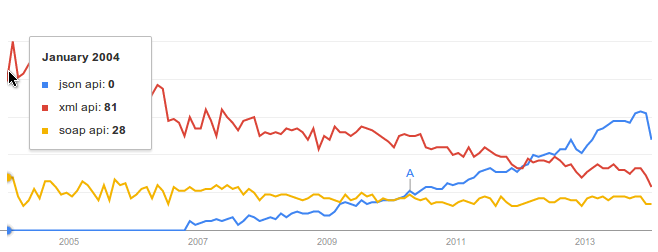
\includegraphics[width=140mm]{images/xml-vs-json-vs-soap-google-trends.png}
\caption{Google Trends for JSON API, XML API, and SOAP API}
\label{fig:googletrends}
\end{figure}

Developers using popular languages and frameworks can very likely parse any valid data format you return to them. You can even interchange data in any of the aforementioned data formats (not including SOAP) quite easily, if you're building a common response object and swapping serializers. It is crucial that when supporting multiple return formats you adhere to the \texttt{Accept} header provided by the Consumer.

Some API architects recommend adding a .json, .xml, or .html file extension to the URL (appended to the Endpoint) for specifying the Content Type to be returned. Unfortunately, with the different extensions added, we've now got different URLs representing the same Resources.

Use the \texttt{Accept} header, which is built into the HTTP spec specifically for this purpose, and if you can't provide data in a format the Consumer requests, reply with a \texttt{406 Not Acceptable} status.


\section{Expected Body Content}

When a Consumer makes a request to the Server, something needs to be returned as a response. Depending on the HTTP Method and Endpoint being requested, the expected response will differ.

\subsubsection{GET /\{collection\}}

When performing a GET request to an entire Collection, the Consumer typically expects an array of Resources to be returned. In the simplest form of HTTP APIs, this consists of a single JSON array containing a homogeneous list of resources.

\begin{verbatim}
[
  {
    "id": "1",
    "name": "John Smith",
    "created": "2014-01-01T12:00:00Z",
    "modified": null
  },
  {
    "id": "2",
    "name": "Jane Doe",
    "created": "2014-01-01T12:01:00Z",
    "modified": null
  }
]
\end{verbatim}

\subsubsection{GET /\{collection\}/\{resource\_id\}}

When performing a GET request for a specific resource, the Consumer is expecting to receive the resource object. In a simple HTTP API, this is just the resource as a top level JSON object.

\begin{verbatim}
{
  "id": "2",
  "name": "Jane Doe",
  "created": "2014-01-01T12:01:00Z",
  "modified": null
}
\end{verbatim}

\subsubsection{POST /\{collection\}}

When performing a POST request to a Collection, the Consumer expects the resource it just created to be returned. In the ideal HTTP API, the object being provided is exactly the same as the object being returned. However, there is very important information being returned to the Consumer which it doesn't already know, such as the \texttt{resource\_id} and other calculated attributes such as timestamps.

\begin{verbatim}
{
  "id": "3",
  "name": "Alice Roberts",
  "created": "2014-01-01T12:02:00Z",
  "modified": null
}
\end{verbatim}

\subsubsection{PUT /\{collection\}/\{resource\_id\}}

The result of a PUT operation is the entirety of the resource that was updated, as the root JSON object.

\begin{verbatim}
{
  "id": "3",
  "name": "Alice Smith",
  "created": "2014-01-01T12:01:00Z",
  "modified": "2014-01-01T12:03:00Z"
}
\end{verbatim}

\subsubsection{PATCH /\{collection\}/\{resource\_id\}}

The result of a PATCH request is exactly the same as the result of a PUT operation. Even though the Consumer may have only acted on some of the attributes, the entire resource is returned.

\begin{verbatim}
{
  "id": "3",
  "name": "Alicia Smith",
  "created": "2014-01-01T12:01:00Z",
  "modified": "2014-01-01T12:04:00Z"
}
\end{verbatim}

\subsubsection{DELETE /\{collection\}/\{resource\_id\}}

This is the easiest of the bodies to deal with. Once a resource is deleted, you simply return an empty document. No need to return information about the deleted resource. Since no body is present, omit the \texttt{Content-Type} header.


\section{JSON Attribute Conventions}

JSON, which stands for \emph{JavaScript Object Notation}, is a subset of JavaScript, and was defined for the purpose of building a language-agnostic data interchange format. It fills mostly the same role that XML was designed to fill, except that it has the side effect of being much more compact, easily deserializing into native objects in most languages, and supporting many different data types (XML technically only supports strings).

That said, there is still quite a bit of freedom that a developer has when representing data using JSON. This section of the book is designed to give you advice for representing data.

\subsection{Consistency between Resources}

Whenever you represent different Resources within the same Collection, each attribute should remain of the same data type. For example, if one Resource has a \texttt{name} attribute which is a String, you shouldn't in a different Resource represent it as an Integer.

There are some exceptions, such as when a value doesn't exist, it can be represented as a \texttt{null}. In general, keeping the attributes of the same data type will make your API easier for consumers to use, especially those using statically typed languages (\emph{JavaScript} and \emph{PHP} are more forgiving in this regard than a language like \emph{C}).

\subsection{Booleans}

It may be tempting to name your Booleans with a prefix or postfix to symbolize the purpose of the attribute. Common examples of this would be to prefix the variable with \texttt{is\_} or end it with \texttt{\_flag}.

This really isn't necessary as attribute names are often self-documenting. For example, if there is an attribute on your User resource called \texttt{administrator}, it should be obvious that using a non-Boolean isn't intended.

Another tip with Booleans is that they should usually be a \emph{positive} or \emph{happy} word, as opposed to their negative counterparts. This will prevent developers form having to figure out a double-negative. For example, use \texttt{enabled} instead of \texttt{disabled}, \texttt{public} instead of \texttt{private}, and even \texttt{keep} instead of \texttt{purge}.

\subsection{Timestamps}

There are a multitude of standards for representing dates and times.

\subsubsection{ISO 8601}

The ideal standard for representing dates is the \textbf{ISO 8601} \cite{ISO8601} standard, and it looks a bit like this:

\begin{verbatim}
"2014-01-10T03:06:17.396Z"
"2014-01-09T22:06:17+05:00"
\end{verbatim}

This format is human readable, lacks redundant information, has variable precision (the microseconds on the end is optional), conveys timezone information (the \texttt{Z} means UTC, but an offset can be provided), and is the most popular of standardized date formats.

\subsubsection{JavaScript Default}

JSON is a subset of JavaScript, and JavaScript does have a default format for parsing dates. To see this format generated, create a new \texttt{Date} object and convert it to a String. The format of these dates looks a little something like this:

\begin{verbatim}
"Thu Jan 09 2014 22:06:17 GMT-0500 (EST)"
\end{verbatim}

Unfortunately this format is a verbose eyesore. Who cares what day of the week it was?

\subsubsection{UNIX Epoch}

If you wanted something much more terse, you could represent the date as the number of seconds since the Unix Epoch, and it can be stored as an integer:

\begin{verbatim}
1389323177396
\end{verbatim}

This format is a bit too terse. As a human looking at it, you have no idea what date and time it represents! Linux and Unix machines and open source languages can parse that format very easily, however developers using \emph{Microsoft} technology will likely be clueless.

\subsubsection{SQL Timestamp}

Here is another common date format. This is what happens when a developer takes a \texttt{TIMESTAMP} directly from a SQL database and outputs it into the response:

\begin{verbatim}
"2014-01-10 03:06:17"
\end{verbatim}

The problem with this format is that it does not convey what timezone the date is in! You may be tempted to use this format, and document the timezone of the server (which we refer to as being \emph{out of band}). However, developers will not remember it, and users of their application will wonder why a newly uploaded image has a modified time of five hours and three seconds ago.

\subsection{Resource Identifiers (IDs)}

Whenever communicating IDs, transfer them as a String (even if they are numeric). Everything a Consumer does with an ID is in string form anyway. If they make a request to the Resource, the ID is concatenated with another String and used as a URL. If the ID is logged, it is written as a String on disk. And unless the Consumer is doing some shady scraping of the API, the ID should never need to have arithmetic performed with it.

Also, if IDs are always sent as a String, deciding to change from a numeric representation to a different format such as a UUID (e.g. \texttt{7d531700-79a5-11e3-979a-a79bcbe406e9}) or a Base62 encoded value (e.g. \texttt{oHg5SJYRHA0}) will result in no code changes on the Consumers end.

\subsection{Nulls}

If most Resources have a particular attribute available, and some do not, you should always provide the attribute in the document with a null value, instead of outright removing the attribute.

This will make things easier for Consumers who won't need to check if a JSON attribute exists before attempting to read it.

\subsection{Arrays}

When representing Resources with attributes which represent an array, you should give the attribute a plural name. This signifies to the developer they should expect more than one value.

When an Array shouldn't have any entries, you should typically return an array with nothing in it, instead of returning a null.

\subsection{Whitespace}

Whitespace, while convenient for a human to read, isn't very beneficial to a Consumer, and incurs some extra networking overhead. It's really up to you to decide if you want to add whitespace to the output.

JSON allows for any number of whitespace between keys and values, but if you are going to add whitespace, use a simple and consistent standard. Two spaces for indentation and a single newline is common practice.

\section{Error Reporting}

Errors are an inevitability of any inter-party communication. Users will fat finger an email address, developers will not read the tiny disclaimer you hid in your API documentation, and a database server will occasionally burst into flame. When this happens, the server will of course return a \textbf{4XX} or \textbf{5XX} HTTP Status Code, but the document body itself should have useful information included.

When designing an error object, there isn't a specific standard that you need to follow. The examples that follow aren't an existing standard, however feel free to use them as a starting point when designing your own errors. Make sure that there is consistency between errors regardless of endpoint.

There are essentially two classes of errors you can account for. The first one is a simple error, where it is easy to point to a specific attribute as being the problem. Let's refer to these as validation errors. The second class of errors are a bit more complex, and may not be easily interpreted by an API Consumer. Let's call these generic errors.

\subsection{Validation Errors}

When an error happens regarding a malformed attribute, provide the Consumer with a reference to the attribute causing the error, as well as a message about what is wrong. Assuming the Consumer is providing a UI for a User to input data, they can display the message for the user to read as well as provide context for the User.

\paragraph{\textbf{Erroneous Request}}

\begin{verbatim}
PUT /v1/users/1

{
  "name": "Rupert Styx",
  "age": "Twenty Eight"
}
\end{verbatim}

\paragraph{\textbf{Error Response}}

\begin{verbatim}
400 Bad Request

{
  "error_human": "Inputs not formatted as expected",
  "error_code": "invalid_attributes",
  "fields": [
    {
      "field": "age",
      "error_human": "Age must be a number between 1 and 100",
      "error_code": "integer_validation"
    }
  ]
}
\end{verbatim}

\subsection{Generic Errors}

When an error occurs which can't be traced back to a single input attribute being incorrect, you'll want to return a more generic error construct.

\paragraph{\textbf{Request}}

\begin{verbatim}
POST /v1/animals

{
  "name": "Mittens",
  "type": "kitten"
}
\end{verbatim}

\paragraph{\textbf{Error Response}}

\begin{verbatim}
503 Service Unavailable

{
  "error_human": "The Database is currently unavailable.",
  "error_code": "database_unavailable"
}
\end{verbatim}

\subsection{Always Handle Server Errors}

Make sure that you catch all errors your server is capable of producing, and \emph{always} return content to the Consumer in the format they are expecting!

This sounds obvious, but it can actually be a lot harder than you think. In PHP, for example, extra care has to be made to catch all errors. By default, PHP and many other web languages/frameworks will return HTML formatted errors.

Consumers will throw all sorts of broken data your way. Experiment with your Server and see what sort of errors you can cause it to produce. Try sending malformed JSON, upload a 100GB file, corrupt the HTTP headers, make 100k concurrent requests, even try removing the underlying code or breaking file permissions and see how your web server handles it.

\subsection{String-Based Error Codes}

In my opinion, there are two types of strings in programming. The first type of string contains human readable text, which includes punctuation and different letter cases and even Unicode symbols. These strings should never be used for comparison. When I program in a language which supports both single and double-quotes for strings, I'll surround these in double quotes.

The other types of strings are computer readable strings. These are much simpler, often used for attributes (you wouldn't use \texttt{First Name} as a JSON key, would you?!), and should be all lowercase and contain underscores (or, camelCase, if you're one of \emph{those} people). These strings could pass as names of variables in most languages. I'll usually surround these strings in single quotes.

Returning to the topic of error codes, it is important to provide the Consumer with \emph{both} a computer readable error code, as well as a human readable error message. The code can be looked up and have logic applied to it by the Consumer. The human readable message can change at any point if a translation changes or any type of rewrite happens.

Many APIs I've seen include the use of numeric error codes. For example, if there was an error with a database transaction being committed, the error code might be \texttt{2091}. A third-party developer working with the API and coming across that error is going to have absolutely no idea what that number means, and will have to go look it up in the API docs. If that message were instead \texttt{database\_transaction\_failure}, the developer is going to have somewhat of a clue as to what just happened and will be able to compensate faster.

The Stripe API \cite[\#Errors]{STRIPEAPI} makes great use of error strings for conveying error codes. One such example is \texttt{expired\_card}, which as a third-party developer, you immediately know that the user-supplied card has expired.


\section{Responses should Resemble Requests}

As a general rule, a Response resource structure should closely resemble the equivalent Request resource. This means that the same attribute names and values are used for Requests as well as Responses.

There are of course a few exceptions. A PATCH, for example, only affects a partial document. A POST won't have certain server-calculated attributes (like an ID or a created timestamp). PATCH and PUTs won't have certain read-only attributes (e.g. created and modified times). These differences in attributes should be minimal when possible.

Whenever dealing with the values of attributes, they should always be the same format. A good philosophy to follow is that request objects should be a strict subset of response objects.

\subsection{Acceptable Discrepancy}

In this example, the differences between the Request and the Response documents are minimal. Some of the values are read-only, and calculated on the server (e.g. \texttt{id}, \texttt{modified}, and \texttt{created}). Some of the attributes have default values (e.g. \texttt{enabled}), which is fine too, as long as these are documented.

\paragraph{\textbf{Request}}

\begin{verbatim}
POST /users

{
  "role": "administrator",
  "name": "Rupert Styx"
}
\end{verbatim}

\paragraph{\textbf{Response}}

\begin{verbatim}
{
  "id": "12",
  "role": "administrator",
  "created": "2014-01-15T02:40:46.049Z",
  "modified": null,
  "name": "Rupert Styx",
  "enabled": true
}
\end{verbatim}

\subsection{Avoidable Discrepancy}

In this example, during a POST to the \texttt{users} endpoint, there is a \texttt{role} attribute, which is a string containing possible user roles, such as \texttt{administrator} or \texttt{moderator}. However, in the response, that same data becomes a Boolean of whether or not the user is an administrator. This increases the amount of attribute names the Consumer needs to keep track of.

\paragraph{\textbf{Request}}

\begin{verbatim}
POST /users

{
  "role": "administrator",
  "name": "Rupert Styx"
}
\end{verbatim}

\paragraph{\textbf{Response}}

\begin{verbatim}
{
  "id": "12",
  "administrator": true,
  "name": "Rupert Styx"
}
\end{verbatim}
